\documentclass[sigconf]{acmart}

\usepackage[english]{babel}
\usepackage{blindtext}

\usepackage{listings}

\newcommand{\rn}[1] {{\textcolor{blue}{RN: {#1}}}}

% Copyright
\renewcommand\footnotetextcopyrightpermission[1]{} % removes footnote with conference info
\setcopyright{none}
%\setcopyright{acmcopyright}
%\setcopyright{acmlicensed}
%\setcopyright{rightsretained}
%\setcopyright{usgov}
%\setcopyright{usgovmixed}
%\setcopyright{cagov}
%\setcopyright{cagovmixed}

\settopmatter{printacmref=false, printccs=false, printfolios=true}

% DOI
\acmDOI{}

% ISBN
\acmISBN{}

%Conference
%\acmConference[Submitted for review to SIGCOMM]{}
%\acmYear{2018}
%\copyrightyear{}

%% {} with no args suppresses printing of the price
\acmPrice{}


\begin{document}
\title{	Sluice: A Network-Wide Model for Programmable Networks}

%\titlenote{Produces the permission block, and copyright information}
%\subtitle{Extended Abstract}

\author{Vikas Natesh$^{ 1}$ \space \space    Pravein Govindan Kannan$^{ 2}$  \space \space Anirudh Sivaraman$^{ 1}$  \space \space Ravi Netravali$^{ 3}$}
% \authornote{Note}
\orcid{1234-5678-9012}
\affiliation{
   \institution{$^{ 1}$New York University  \quad \quad \quad $^{ 2}$National University of Singapore  \quad \quad \quad $^{ 3}$University of California, Los Angeles}
%   \streetaddress{Address}
%   \city{City} 
%   \state{State} 
%   \postcode{Zipcode}
 }
% \email{email@domain.com}

% The default list of authors is too long for headers}
\renewcommand{\shortauthors}{V. Natesh. et al.}

%\begin{abstract}
  %  \blindtext
%\end{abstract}

\maketitle

\section{Introduction}
The last several years have seen the emergence of programmable network devices
including both programmable switching chips and programmable network interface
cards (NICs). Along with the rise of x86-based packet processing for
middleboxes and virtual switches, these trends point towards a future where the
entire network will be programmable. The benefits of network programmability
range from commercial use cases such as network virtualization implemented on
the programmable Open vSwitch platform to more recent projects that implement
packet scheduling, measurement, and application offload of niche applications
on programmable switches.

Benefits are clear, but are difficult to reap as
programming network as a whole remains challenging. Current programming languages target individual
network devices, e.g., P4 for the Tofino programmable switching chip and the
Netronome programmable NIC. However, at present, there is no unified
programming model to express and implement general functionality at the level
of an entire network, without having to individually program each network
device.

Maple was an early example of a network-wide programming model designed
for OpenFlow switches. Maple automatically divided functionality between a
stateless component running on switches and a stateful component running on the
network's controller. SNAP is a more recent example of network-wide
programming; unlike Maple, it additionally offloads stateful functionality to
switches by leveraging stateful processing available in programmable switches. However, both Maple
and SNAP cannot express programmable-switch functionality that affects network
performance at fine time scales \rn{is there a short `why' for this?}, e.g.,
packet scheduling, congestion control, fine-grained measurement of microbursts,
and load balancing. In other words, Maple and SNAP generate highly optimized
code, but are restricted in what they can express.

This demo presents \textbf{Sluice}, a programming model that takes a high-level
specification of a network program and compiles it into runnable code that can
be launched directly on the programmable devices of a network. In contrast to
prior network-wide programming models like SNAP and Maple, Sluice aims to be
more general \rn{should directly contrast with Maple/SNAP being
coarse-grained}, but potentially at the cost of quality of generated code.
Sluice endows network operators with the ability to design and deploy large
network programs for various functions such as scheduling, measurement, and
application offloading.  The benefits of Sluice can be summarized as follows:\\
\indent - Sluice provides the same functionality as P4 but makes it easier to
program the data plane of an entire network. \\
\indent - Sluice automatically reduces the amount of boilerplate code needed to
write an equivalent program in P4. For instance, the 9 line traffic matrix
sluice program translates into over 200 lines of P4 code.

We demonstrate Sluice's functionality and ease of use
via two examples: traffic matrix generation for network analysis and a
streaming join-filter operation.
\begin{figure}[tp]
\centering
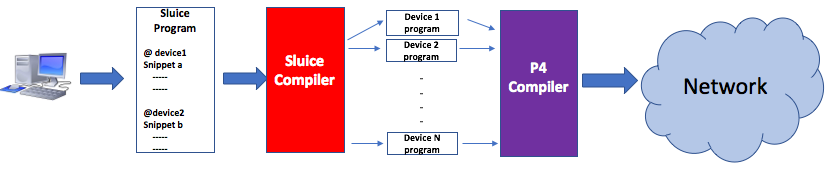
\includegraphics[width=80mm,scale=0.7]{figures/sluice_workflow.png}
\caption{Sluice Workflow}
\vspace{-8mm}
\end{figure}
\vspace{-4mm}

\section{Sluice Design}
In the Sluice model, a network-wide program consists of high-level code
\textit{snippets} annotated by the operator to run on particular devices in a
network. The code in each snippet is to be executed on packets arriving at its
corresponding device. Snippets support a variety of operations:
read-from/write-to packets; arithmetic using packet data, local variables, or
stateful register arrays; and control flow statements. To handle computation on
custom packet headers not supported by default (ip/tcp/udp/eth), users may
define packet declarations similar to C structs. An optional annotation in the
declaration, the parser condition, automatically generates a header parser.
This lets the user restrict snippets to operate on specific flows or IP address
ranges. Sluice programs may also import device-specific variables/attributes
for use in code snippets.

Figure 1 describes the Sluice workflow. The compiler translates each snippet of
a sluice program into a device-specific program. After initial parsing, lines of code in
the snippet are decomposed into a directed acyclic graph (DAG) that maps
dependencies between variables in each snippet \rn{I'm confused. Isn't each
node a snippet? Or are you breaking a snippet into smaller components?}. This
graph is then passed to the backend of the compiler that generates the
corresponding P4 program for that device, for example bmv2 or
Tofino.\footnote{Currently we only support bmv2 but plan to support more
devices.} 

%Example of citation here\cite{floyd1993random, stoica2001chord}



\section{Demonstrations}
 
\subsection{Traffic Matrix}

Figure 2 displays the Mininet network topology for our traffic matrix demo.
Packets are sent over UDP from each host to all other hosts according to a
poisson traffic model with mean inter-arrival time of 0.5 seconds. The codelet
below is our Sluice program with a single snippet \textit{traffic\_example}
that is launched on all switches of the network. To run the simulation, the
user passes the Sluice program and network topology to the compiler. The
compiler generates P4 code to run on each switch as well as control plane table
entries for routing packets through the topology.

\begin{lstlisting}[language=Python, basicstyle=\scriptsize]
import device psa;

packet p: udp(srcPort:1234)
  nhops : bit<32>;

@ bmv2 : ;
snippet traffic_example()
  persistent cnt : bit<32>[10];
  cnt[psa.ingress_port] = cnt[psa.ingress_port] + 1;
  p.nhops = p.nhops + 1;
\end{lstlisting}

This demo shows how a simple Sluice program can be used to enable each switch
to measure link usage for a specific flow of user-defined packets on UDP
srcPort 1234. Each packet \textit{p} contains a custom header \textit{nhops}
that is incremented each time the packet enters a switch to inform the
receiving host of the number of hops the packet took. Each switch maintains a
stateful register counter \textit{cnt}, indexed by switch ingress port, that
tracks how many packets have entered through that ingress port. Aggregated over
all switches, these counters data represent a matrix measuring each link's
usage in the network at a given time. This matrix (residing on the whole
network) is then queried once every second from the control plane to generate
time-series plots of link-utilization for each link. Figure 3 displays the
histogram of packet rates on link s1-s3 after collecting data for 3 minutes.
The expected distribution of packet rates \textit{poisson}($\mu = 2$
packets/sec) is also plotted to confirm the accuracy of the Mininet emulation.

\begin{figure}[tp]
\centering
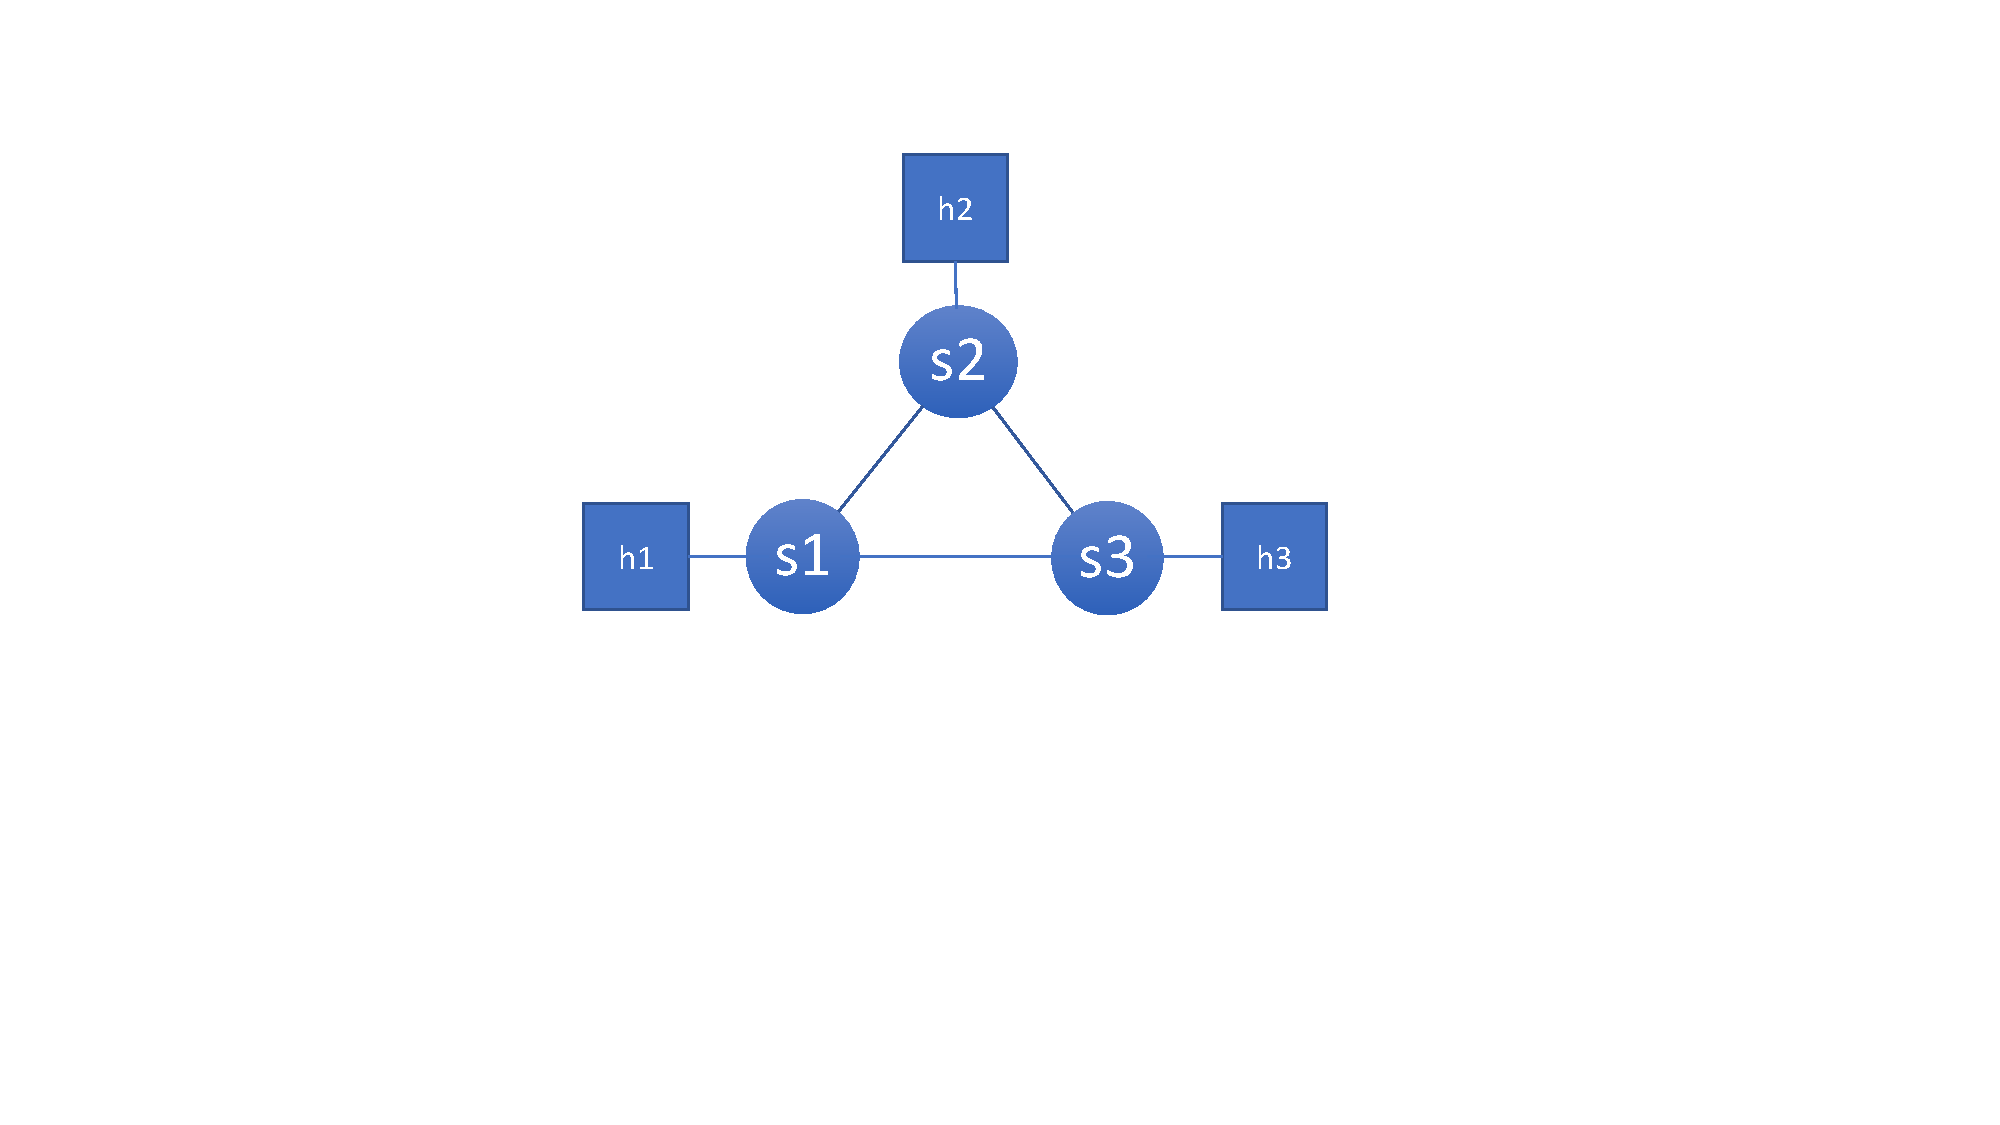
\includegraphics[width=40mm,scale=0.7]{figures/traf_mat_topo}
\caption{Topology For Traffic Matrix Demo}
\end{figure}


\begin{figure}[tp]
\centering
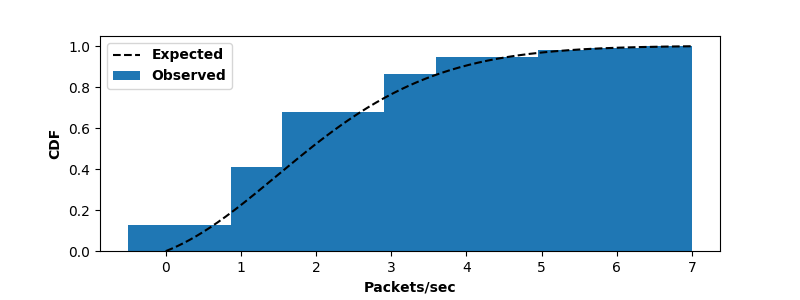
\includegraphics[width=80mm,scale=0.7]{figures/exp_obs_cdf}
\caption{CDF of Packet Rate on link s1-s3}
\end{figure}
  
\subsection{Stream processing}
This example demonstrates a simple join-filter operation between two streams of
tuples. A stream is an unbounded table where a packet represents a tuple of
data (\textit{ad\_id, impression\_time, click\_time}) enclosed in a custom
header. The topology in Figure 4 describes the data flow and shows how an
operator query runs on the switches of the network. Host 1 sends a stream of ad
impressions while Host 2 sends a stream of ad clicks. The two streams are
joined on the \textit{ad\_id} field at s1 and filtered on the \textit{ad\_id}
field at s2 and the result is sent to h3. 

\begin{figure}[tp]
\centering
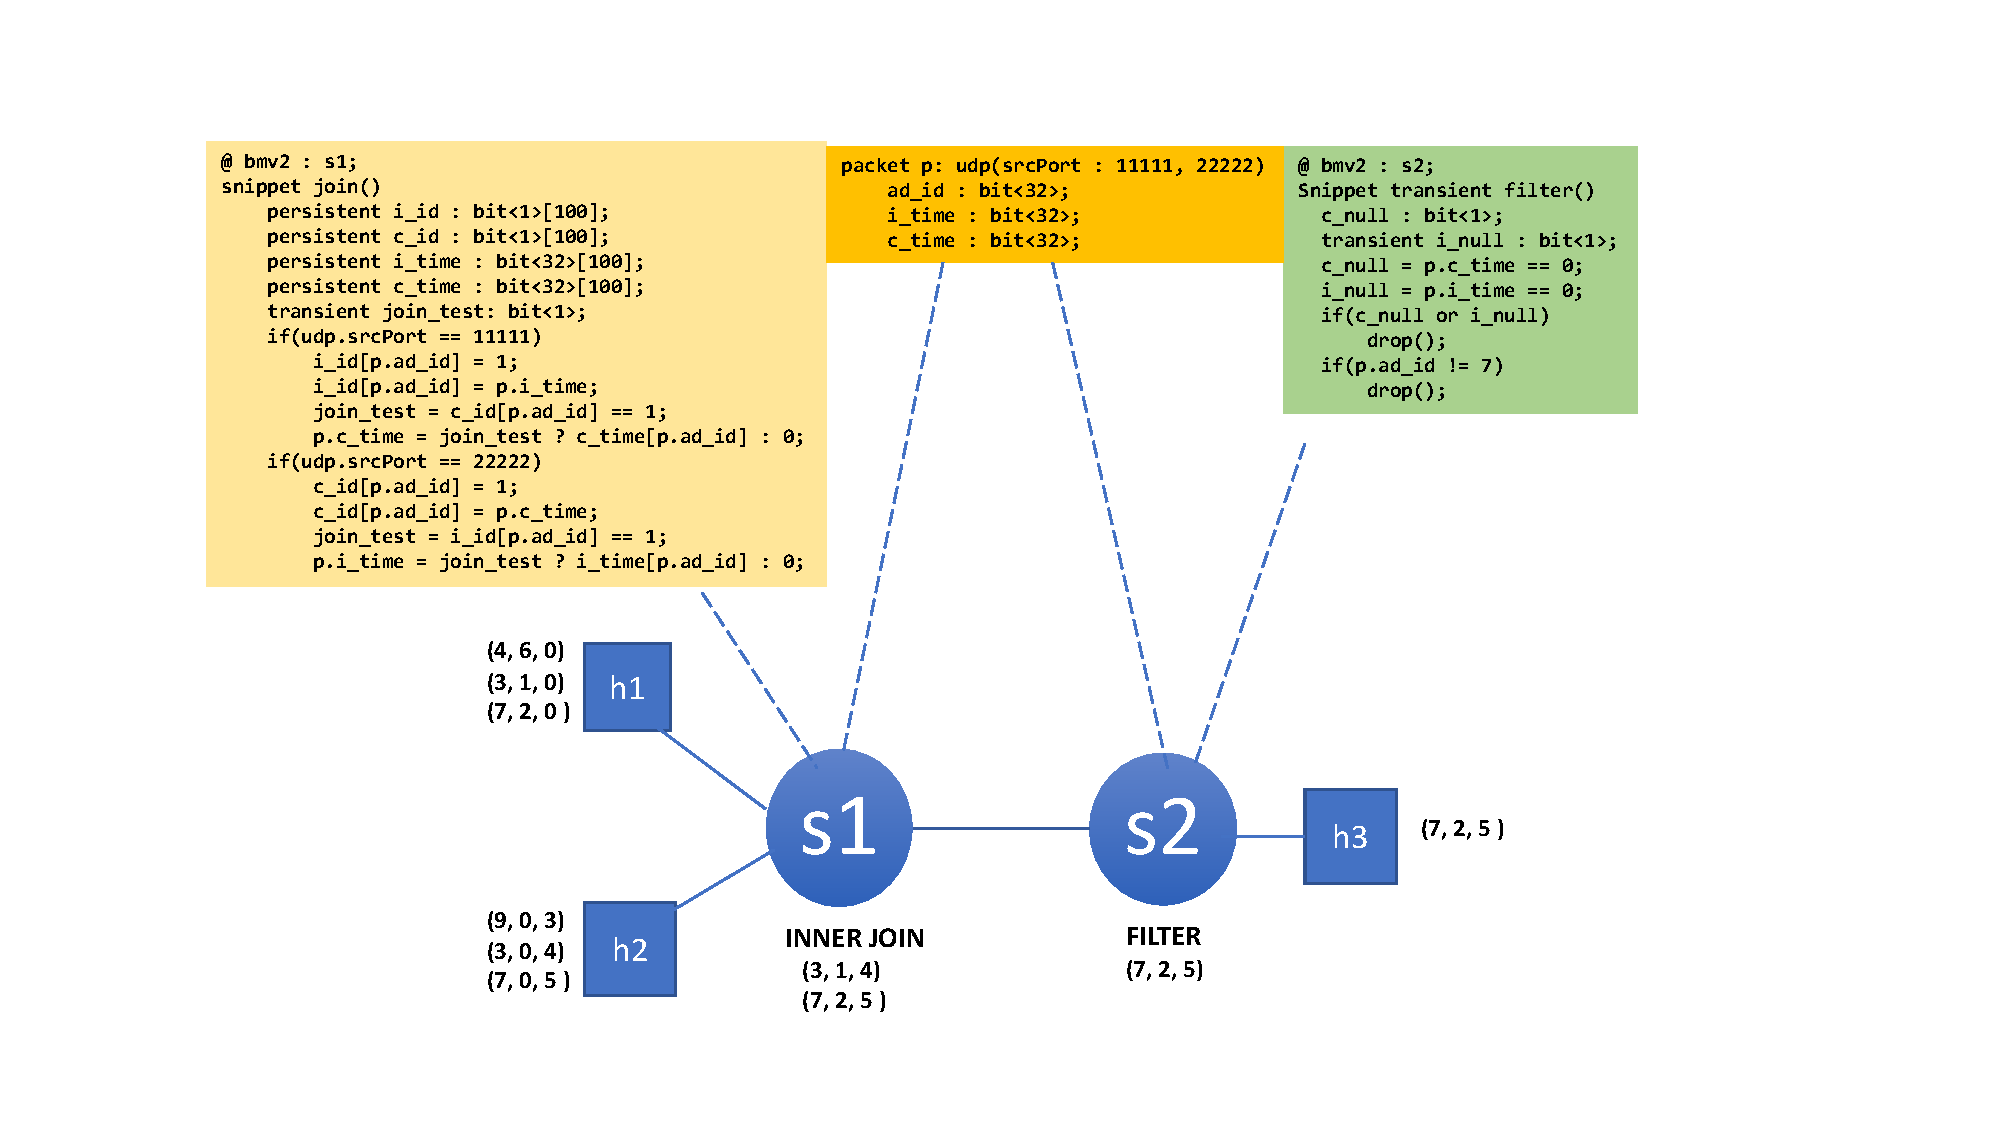
\includegraphics[width=80mm,scale=0.7]{figures/streaming_example}
\caption{streaming example topology, data flow, and code placement on switches}
\vspace{-5mm}
\end{figure}
\vspace{-5mm}


\section{Future Work}
\textbf{An optimizing Sluice compiler.} We envision using the dependency DAG to
provide several automatic optimizations or code transformations. For example,
it is possible that certain lines of code in a snippet cannot be run on the
device annotated by the operator, e.g., programmable switching chips have
limited support for floating point or complex string operations. Code
containing such features must be moved to the control plane or an end host data
plane while at the same time, preserving the original program semantics
intended by the operator. Doing this automatically would free the Sluice
programmer from reasoning about these semantics.

\textbf{Supporting multi-tenancy.} Another area of future work is allowing
Sluice \rn{would this really be a change to Sluice? Or would this be using
Sluice to do something else?} to support multiple tenants with their own Sluice
programs running on their own virtual networks overlayed on the same physical
topology. If each tenant wants to run their own network-wide program on their
virtual topology, the network operator will need to merge all these into one
data plane implementation that runs on the entire physical network. Extending
Sluice to support this multi-tenancy use case would allow us to provide the
same benefits to the data plane that multi-tenant network
virtualization~\cite{nvp} provided for the control plane.

\section{References}


\bibliographystyle{ACM-Reference-Format}
\bibliography{reference}

\end{document}
